
\documentclass[11pt,letterpaper]{article}
\usepackage[margin=0.9in]{geometry}
\usepackage[T1]{fontenc}
\usepackage{amsmath,amssymb,graphicx,booktabs,array,url}
\usepackage[hidelinks]{hyperref}
\hypersetup{pdftitle={NeST-Com: Supplementary Configurations and Results},pdfauthor={Anonymous Authors}}
\setlength{\parindent}{0pt}\setlength{\parskip}{6pt}\emergencystretch=2em
\newcommand{\Dc}{D_c}
\begin{document}
\begin{center}\Large\bfseries NeST-Com: Fixed-Budget Next-Scale Token Communication\\[4pt]\large Supplementary Configurations and Results\end{center}
\section*{S1. Configuration and calibration}
This supplement collects the completed experiments supporting the accompanying letter. It reformats existing results; it adds no model inference, wireless trial, metric evaluation, training, or statistical resampling. All differences below retain the original comparison direction and population.

\textbf{Models and training.} NeST and WHOLE share the VAR tokenizer, null-class prior, entropy coder, and adapted image decoder $\Dc$. Its adaptation uses 20\,000 ImageNet training images and continuous, fully quantized, and prefix-completion-interpolated latents. The convolutional Latent JSCC uses MSE, LPIPS, and latent-consistency losses and the same decoder; its final checkpoint is at 100k updates. SwinJSCC uses the same 20\,000 images, $256\times256$ input, paid side information, and a final 200k-update checkpoint. The Swin selection record reports \texttt{BUDGET\_CAP\_WHILE\_IMPROVING}; no claim of full convergence is made. The selected checkpoint, calibration history, stopping checks, and original training plots are available through the linked index.

\textbf{Ada adaptation.} Ada retains LlamaGen-L/VQ16 and genuine autoregressive prefix arithmetic coding. A fixed ConvNeXt predicts the class at TX; its 10-bit ID travels in the protected body, giving $b+39\leq k_a$. RX uses the recovered class and prefix. All 1--256 independently terminated prefixes are eligible. Main-curve tail generation uses CFG=4, temperature 1, top-$k=2000$, top-$p=1$, FP32 with TF32 off. The fixed single-frame adaptation does not reproduce the original long-term average-budget controller or ARQ. At N1024/19~dB all 256 tokens are sent; remaining source capacity therefore does not indicate fitting failure.

\textbf{Calibration.} The 100-image pilot uses one channel realization per source. Final evaluation uses all 1000 calibration images with three realizations per source, including fixed-gray failures. Selection maximizes DINOv2 cosine, first averaging realizations and then equally weighting sources. Exact ties use the frozen candidate order. DINO-based selection is related to feature-based evaluation; the controlled interventions separately examine the mechanism.

N1024 target screening starts at scales 7--9 and includes full-scale $(10,0)$ candidates in final evaluation. N512 screens all 7 WHOLE and 25 Quarter targets against 12 MCSs: $\log_2 M\in\{2,4,6\}$ and rates $\{1/2,2/3,3/4,5/6\}$. Each method/SNR advances the top three and a maximum-endpoint QPSK rate-1/2 anchor. Ada uses the same N512 MCS pool and up to 256 tokens. Each budget is independently calibrated; its results describe separately selected systems, rather than an isolated causal change in budget or representation order.

\href{https://github.com/daiqizai/var-comm/blob/2c303b615f73edd0a7a971308c0df8bd5bb885d0/results/baseline_strength_20261011/Swin_1to19/selected_checkpoint.json}{Swin checkpoint and training status}; \href{https://github.com/daiqizai/var-comm/blob/2c303b615f73edd0a7a971308c0df8bd5bb885d0/results/baseline_strength_20261011/training_figures_v1/training_calibration_curves.pdf}{training and calibration curves}; \href{https://github.com/daiqizai/var-comm/blob/2c303b615f73edd0a7a971308c0df8bd5bb885d0/results/nestcom_n512_20261028_v1/protocol.json}{N512 frozen protocol}.

\clearpage\section*{S2. Statistical populations and reception accounting}
The main population is common500; Kodak has 24 sources. The endpoint, receiver, and E1/E2 controls use the existing fixed 100-source subset, not a new independent blind test. Full source IDs, preprocessing identities, and native pixel hashes join the records. Three original outcomes are averaged within a source before equal-source means and paired differences. Percentile 95\% intervals use 10\,000 source resamples; they are pointwise, not simultaneous intervals. Marginal intervals are never subtracted.

N512 methods share the registered source/repeat AWGN identities. N1024 preserves historical noise identities and is not presented as sharing noise across every method or budget. E1/E2 reuse those actual reception states; receiver counterfactuals are not new wireless frames. The 100-source bank is matched by its complete source order, not sliced from the 500-source bank. Both registered banks use seed 2026100701. Full hashes and source orders remain in the statistical identity files.

\textbf{Main matched-SNR failures.} N1024 has no rejected or failed reconstructions in 1500 trials per method/SNR; continuous Latent JSCC has no discrete CRC rejection. N512 failures below are body-CRC rejections, retained as fixed gray in all means. Header, parser, and source-decoder rejection counts are zero. No evaluated N512 source requires a NULL frame.
\begin{center}\begin{tabular}{lrrrr}\toprule
Method & 4 dB & 10 dB & 19 dB & Trials per SNR\\\midrule
NeST & 4 & 1 & 0 & 1500\\
WHOLE & 7 & 0 & 0 & 1500\\
Ada & 5 & 0 & 0 & 1500\\\bottomrule
\end{tabular}\end{center}
\textbf{No-feasible-endpoint behavior.} The actual implementations differ. N512 sends a paid NULL profile and two zero payload bits through the complete 68+444-symbol frame, returning gray. N1024 raises an execution error when no independently terminated legal stream fits; this case did not occur in its evaluated sources. The revision preserves both frozen implementations. Seven synthetic CPU checks of the original source-selection/RX-projection functions verify no-fit and ordinary-fit branches, with no PHY or model calls. Source hashes and line ranges are in the implementation audit; these checks do not constitute new wireless qualification.

\textbf{Granularity and receiver controls.} Mean terminated-length checks are 3.55/5.55/9.49/17.58 for Whole/Half/Quarter/Eighth. They compare already terminated streams, not extra model forwards or measured latency. Quarter is a predefined configuration, not a demonstrated optimum. The A0/B0/C0 differences are ordered interventions on the same prefixes; they are not a universal percentage decomposition. A0 still performs prior completion. At the final scale C0 and B0 coincide because no finer context is used.

\clearpage\section*{S3. Ada tail sensitivity: $N=512$, 4 dB}
All entries use the same 100 sources and three original repetitions (300 logical results per arm). Each cell is a mean or direct paired difference with its 95\% source-bootstrap interval. Higher PSNR/CLIP-I and lower LPIPS/DreamSim are favorable.
\subsection*{Absolute metrics}
\begin{center}\small\setlength{\tabcolsep}{7pt}\renewcommand{\arraystretch}{1.55}
\begin{tabular}{lccc}
\toprule
Metric & Ada sampling & Ada argmax & NeST\\\midrule
PSNR (dB) $\uparrow$ & \shortstack{10.984\\{}[10.574, 11.410]} & \shortstack{10.509\\{}[10.099, 10.933]} & \shortstack{15.141\\{}[14.621, 15.673]}\\
LPIPS $\downarrow$ & \shortstack{0.5610\\{}[0.5457, 0.5759]} & \shortstack{0.6033\\{}[0.5857, 0.6209]} & \shortstack{0.3668\\{}[0.3511, 0.3823]}\\
DreamSim $\downarrow$ & \shortstack{0.3797\\{}[0.3523, 0.4071]} & \shortstack{0.4247\\{}[0.3966, 0.4534]} & \shortstack{0.2786\\{}[0.2591, 0.2981]}\\
CLIP-I $\uparrow$ & \shortstack{0.7922\\{}[0.7740, 0.8095]} & \shortstack{0.7661\\{}[0.7466, 0.7851]} & \shortstack{0.7658\\{}[0.7468, 0.7855]}\\
\bottomrule\end{tabular}\end{center}
\subsection*{Direct source-paired differences}
\begin{center}\small\setlength{\tabcolsep}{7pt}\renewcommand{\arraystretch}{1.55}
\begin{tabular}{lccc}
\toprule
Metric & \shortstack{Argmax minus\\sampling} & \shortstack{NeST minus\\argmax} & \shortstack{NeST minus\\sampling}\\\midrule
PSNR (dB) $\uparrow$ & \shortstack{-0.475\\{}[-0.801, -0.152]} & \shortstack{4.632\\{}[4.183, 5.093]} & \shortstack{4.157\\{}[3.772, 4.558]}\\
LPIPS $\downarrow$ & \shortstack{0.0423\\{}[0.0294, 0.0555]} & \shortstack{-0.2365\\{}[-0.2567, -0.2167]} & \shortstack{-0.1942\\{}[-0.2100, -0.1789]}\\
DreamSim $\downarrow$ & \shortstack{0.0450\\{}[0.0282, 0.0621]} & \shortstack{-0.1461\\{}[-0.1709, -0.1218]} & \shortstack{-0.1010\\{}[-0.1248, -0.0769]}\\
CLIP-I $\uparrow$ & \shortstack{-0.0261\\{}[-0.0378, -0.0143]} & \shortstack{-0.0003\\{}[-0.0194, 0.0185]} & \shortstack{-0.0263\\{}[-0.0449, -0.0078]}\\
\bottomrule\end{tabular}\end{center}
Fixed-gray counts per 300: Ada-sampling: 0, Ada-argmax: 0, NeST: 1.
The deterministic tail lowers Ada PSNR and worsens its three feature metrics relative to sampling. NeST retains higher PSNR and lower LPIPS/DreamSim than argmax; the CLIP-I difference interval crosses zero. The sampling configuration remains the main baseline.
Only unreceived-tail token selection changes. Context/KV is rebuilt from the actual received prefix and follows each new greedy token. The paid class, CFG composition, entropy-decoding conditional CDF, model, decoder, and numerical route remain fixed. No sampling-tail KV is reused. Full-token receptions reuse the existing output exactly; failed/NULL inputs remain gray.
\clearpage\section*{S3. Ada tail sensitivity: $N=512$, 10 dB}
All entries use the same 100 sources and three original repetitions (300 logical results per arm). Each cell is a mean or direct paired difference with its 95\% source-bootstrap interval. Higher PSNR/CLIP-I and lower LPIPS/DreamSim are favorable.
\subsection*{Absolute metrics}
\begin{center}\small\setlength{\tabcolsep}{7pt}\renewcommand{\arraystretch}{1.55}
\begin{tabular}{lccc}
\toprule
Metric & Ada sampling & Ada argmax & NeST\\\midrule
PSNR (dB) $\uparrow$ & \shortstack{12.878\\{}[12.384, 13.398]} & \shortstack{12.227\\{}[11.738, 12.751]} & \shortstack{16.827\\{}[16.313, 17.347]}\\
LPIPS $\downarrow$ & \shortstack{0.4121\\{}[0.3975, 0.4266]} & \shortstack{0.4416\\{}[0.4237, 0.4598]} & \shortstack{0.2818\\{}[0.2683, 0.2955]}\\
DreamSim $\downarrow$ & \shortstack{0.2511\\{}[0.2296, 0.2728]} & \shortstack{0.2856\\{}[0.2627, 0.3098]} & \shortstack{0.1955\\{}[0.1797, 0.2123]}\\
CLIP-I $\uparrow$ & \shortstack{0.8337\\{}[0.8170, 0.8502]} & \shortstack{0.8105\\{}[0.7929, 0.8278]} & \shortstack{0.8208\\{}[0.8028, 0.8386]}\\
\bottomrule\end{tabular}\end{center}
\subsection*{Direct source-paired differences}
\begin{center}\small\setlength{\tabcolsep}{7pt}\renewcommand{\arraystretch}{1.55}
\begin{tabular}{lccc}
\toprule
Metric & \shortstack{Argmax minus\\sampling} & \shortstack{NeST minus\\argmax} & \shortstack{NeST minus\\sampling}\\\midrule
PSNR (dB) $\uparrow$ & \shortstack{-0.651\\{}[-0.984, -0.338]} & \shortstack{4.600\\{}[4.188, 5.018]} & \shortstack{3.949\\{}[3.566, 4.348]}\\
LPIPS $\downarrow$ & \shortstack{0.0296\\{}[0.0201, 0.0394]} & \shortstack{-0.1598\\{}[-0.1754, -0.1439]} & \shortstack{-0.1302\\{}[-0.1429, -0.1178]}\\
DreamSim $\downarrow$ & \shortstack{0.0345\\{}[0.0232, 0.0461]} & \shortstack{-0.0901\\{}[-0.1120, -0.0689]} & \shortstack{-0.0556\\{}[-0.0760, -0.0360]}\\
CLIP-I $\uparrow$ & \shortstack{-0.0231\\{}[-0.0337, -0.0128]} & \shortstack{0.0102\\{}[-0.0072, 0.0280]} & \shortstack{-0.0129\\{}[-0.0300, 0.0039]}\\
\bottomrule\end{tabular}\end{center}
Fixed-gray counts per 300: Ada-sampling: 0, Ada-argmax: 0, NeST: 1.
The deterministic tail lowers Ada PSNR and worsens its three feature metrics relative to sampling. NeST retains higher PSNR and lower LPIPS/DreamSim than argmax; the CLIP-I difference interval crosses zero. The sampling configuration remains the main baseline.
Only unreceived-tail token selection changes. Context/KV is rebuilt from the actual received prefix and follows each new greedy token. The paid class, CFG composition, entropy-decoding conditional CDF, model, decoder, and numerical route remain fixed. No sampling-tail KV is reused. Full-token receptions reuse the existing output exactly; failed/NULL inputs remain gray.
\clearpage\section*{S3. Ada tail sensitivity: $N=1024$, 10 dB}
All entries use the same 100 sources and three original repetitions (300 logical results per arm). Each cell is a mean or direct paired difference with its 95\% source-bootstrap interval. Higher PSNR/CLIP-I and lower LPIPS/DreamSim are favorable.
\subsection*{Absolute metrics}
\begin{center}\small\setlength{\tabcolsep}{7pt}\renewcommand{\arraystretch}{1.55}
\begin{tabular}{lccc}
\toprule
Metric & Ada sampling & Ada argmax & NeST\\\midrule
PSNR (dB) $\uparrow$ & \shortstack{19.200\\{}[18.592, 19.824]} & \shortstack{19.044\\{}[18.403, 19.698]} & \shortstack{19.612\\{}[19.083, 20.146]}\\
LPIPS $\downarrow$ & \shortstack{0.1717\\{}[0.1596, 0.1845]} & \shortstack{0.1755\\{}[0.1625, 0.1890]} & \shortstack{0.1752\\{}[0.1653, 0.1851]}\\
DreamSim $\downarrow$ & \shortstack{0.0863\\{}[0.0795, 0.0933]} & \shortstack{0.0899\\{}[0.0823, 0.0978]} & \shortstack{0.1077\\{}[0.1000, 0.1157]}\\
CLIP-I $\uparrow$ & \shortstack{0.8897\\{}[0.8764, 0.9023]} & \shortstack{0.8884\\{}[0.8751, 0.9008]} & \shortstack{0.8759\\{}[0.8607, 0.8905]}\\
\bottomrule\end{tabular}\end{center}
\subsection*{Direct source-paired differences}
\begin{center}\small\setlength{\tabcolsep}{7pt}\renewcommand{\arraystretch}{1.55}
\begin{tabular}{lccc}
\toprule
Metric & \shortstack{Argmax minus\\sampling} & \shortstack{NeST minus\\argmax} & \shortstack{NeST minus\\sampling}\\\midrule
PSNR (dB) $\uparrow$ & \shortstack{-0.156\\{}[-0.369, 0.057]} & \shortstack{0.568\\{}[0.246, 0.902]} & \shortstack{0.412\\{}[0.157, 0.677]}\\
LPIPS $\downarrow$ & \shortstack{0.0038\\{}[0.0007, 0.0071]} & \shortstack{-0.0003\\{}[-0.0072, 0.0062]} & \shortstack{0.0034\\{}[-0.0021, 0.0089]}\\
DreamSim $\downarrow$ & \shortstack{0.0036\\{}[0.0010, 0.0060]} & \shortstack{0.0178\\{}[0.0129, 0.0229]} & \shortstack{0.0214\\{}[0.0167, 0.0262]}\\
CLIP-I $\uparrow$ & \shortstack{-0.0013\\{}[-0.0052, 0.0025]} & \shortstack{-0.0124\\{}[-0.0222, -0.0025]} & \shortstack{-0.0137\\{}[-0.0235, -0.0038]}\\
\bottomrule\end{tabular}\end{center}
Fixed-gray counts per 300: Ada-sampling: 0, Ada-argmax: 0, NeST: 0.
The argmax PSNR difference from sampling includes zero, while DreamSim becomes worse. NeST retains higher PSNR than argmax; Ada argmax retains better DreamSim and CLIP-I, and the LPIPS interval crosses zero. Decoding sensitivity does not remove other complete-system differences.
Only unreceived-tail token selection changes. Context/KV is rebuilt from the actual received prefix and follows each new greedy token. The paid class, CFG composition, entropy-decoding conditional CDF, model, decoder, and numerical route remain fixed. No sampling-tail KV is reused. Full-token receptions reuse the existing output exactly; failed/NULL inputs remain gray.

\clearpage\section*{S4. Completion versus direct coarse decoding}
R0 decodes $\Dc(\sum_{s=1}^{m}C_s(q_s))$ from the actual received WHOLE prefix. R1 is the existing VAR-completed reconstruction of that same prefix. Both retain the original ten-scale indexing, scale-dependent residual transforms, full latent grid, frozen adapted $\Dc$, clipping, and metric preprocessing. Unreceived scales contribute nothing to R0; codebook ID zero is not used as zero contribution. Neither arm uses unsent source tokens or a continuous source latent. This is distinct from A0/B0/C0, which intervene on received boundary-token use.

\subsection*{$N=512$, 4 dB: 100 sources, 300 results per arm}
\begin{center}\small\setlength{\tabcolsep}{7pt}\renewcommand{\arraystretch}{1.55}
\begin{tabular}{lccc}
\toprule
Metric & R0 coarse & R1 completed & R1 minus R0\\\midrule
PSNR (dB) $\uparrow$ & \shortstack{14.787\\{}[14.293, 15.296]} & \shortstack{14.813\\{}[14.261, 15.383]} & \shortstack{0.026\\{}[-0.204, 0.271]}\\
LPIPS $\downarrow$ & \shortstack{0.6612\\{}[0.6376, 0.6843]} & \shortstack{0.3960\\{}[0.3752, 0.4172]} & \shortstack{-0.2652\\{}[-0.2806, -0.2500]}\\
DreamSim $\downarrow$ & \shortstack{0.7369\\{}[0.7154, 0.7575]} & \shortstack{0.3166\\{}[0.2915, 0.3421]} & \shortstack{-0.4204\\{}[-0.4488, -0.3925]}\\
CLIP-I $\uparrow$ & \shortstack{0.5493\\{}[0.5337, 0.5649]} & \shortstack{0.7521\\{}[0.7303, 0.7737]} & \shortstack{0.2028\\{}[0.1837, 0.2218]}\\
\bottomrule\end{tabular}\end{center}
Fixed-gray count per arm: 3.
\subsection*{$N=512$, 10 dB: 100 sources, 300 results per arm}
\begin{center}\small\setlength{\tabcolsep}{7pt}\renewcommand{\arraystretch}{1.55}
\begin{tabular}{lccc}
\toprule
Metric & R0 coarse & R1 completed & R1 minus R0\\\midrule
PSNR (dB) $\uparrow$ & \shortstack{15.722\\{}[15.235, 16.209]} & \shortstack{16.493\\{}[15.993, 17.004]} & \shortstack{0.771\\{}[0.563, 0.986]}\\
LPIPS $\downarrow$ & \shortstack{0.5581\\{}[0.5388, 0.5771]} & \shortstack{0.2943\\{}[0.2817, 0.3068]} & \shortstack{-0.2638\\{}[-0.2774, -0.2504]}\\
DreamSim $\downarrow$ & \shortstack{0.6574\\{}[0.6335, 0.6804]} & \shortstack{0.2055\\{}[0.1897, 0.2216]} & \shortstack{-0.4519\\{}[-0.4790, -0.4248]}\\
CLIP-I $\uparrow$ & \shortstack{0.5748\\{}[0.5574, 0.5924]} & \shortstack{0.8150\\{}[0.7965, 0.8338]} & \shortstack{0.2403\\{}[0.2206, 0.2595]}\\
\bottomrule\end{tabular}\end{center}
Fixed-gray count per arm: 0.
Completion improves all three feature metrics at both points; PSNR improves clearly at 10~dB, while its 4~dB interval includes zero. These results concern completion in the existing adapted receiver, including its decoder training.

\clearpage\section*{S5. Additional results and processing cost}
\textbf{N2048.} On 100 sources, the existing experiment uses two paid 1024-symbol subframes. Complete representations at 19~dB give NeST $+1.806$~dB PSNR over ARPC, but worse DISTS\footnote{K. Ding, K. Ma, S. Wang, and E. P. Simoncelli, ``Image quality assessment: Unifying structure and texture similarity,'' \emph{IEEE Trans. Pattern Anal. Mach. Intell.}, vol. 44, no. 5, pp. 2567--2581, May 2022.}: $+0.0054\,[0.0024,0.0086]$. DISTS is an additional perceptual measure in this historical experiment, not a replacement for the four main metrics.

\textbf{SNR mismatch.} With both WHOLE/PARTIAL transmit policies fixed at 10~dB and RX using the true noise variance, all 300 receptions per method on 100 sources are rejected at 8~dB. All succeed at 10 and 12~dB; for each source and method the recovered prefix and reconstruction are identical at those two points. PARTIAL exceeds WHOLE by $0.660\,[0.515,0.814]$~dB PSNR. These tested points do not locate the rejection threshold or measure the steepness of the 8--10~dB transition.

\textbf{Processing cost.} The following software times are from an RTX PRO~6000 with six CPU cores, batch one, 16 development images, and three measured repetitions after warm-up. They are measured processing times, distinct from the count of length checks. Ada was not timed under this protocol.
\begin{center}\small\begin{tabular}{llrrr}\toprule
Method & SNR (dB) & TX mean (ms) & RX mean (ms) & Total mean (ms)\\\midrule

NeST & 4 & 185.50 & 358.71 & 544.21\\
NeST & 10 & 220.89 & 398.82 & 619.71\\
NeST & 19 & 302.35 & 472.27 & 774.62\\
Latent JSCC & 4 & 16.15 & 24.50 & 40.65\\
Latent JSCC & 10 & 17.97 & 24.51 & 42.48\\
Latent JSCC & 19 & 16.99 & 24.43 & 41.42\\
SwinJSCC & 4 & 24.02 & 18.59 & 42.61\\
SwinJSCC & 10 & 24.81 & 19.89 & 44.69\\
SwinJSCC & 19 & 24.90 & 18.43 & 43.32\\
BPG + LDPC & 4 & 2285.93 & 18.50 & 2304.43\\
BPG + LDPC & 10 & 2269.87 & 23.15 & 2293.01\\
BPG + LDPC & 19 & 2269.24 & 27.26 & 2296.50\\
ARPC + LDPC-QAM & 4 & 716.44 & 719.05 & 1435.49\\
ARPC + LDPC-QAM & 10 & 719.12 & 801.18 & 1520.30\\
ARPC + LDPC-QAM & 19 & 718.19 & 868.69 & 1586.89\\
\bottomrule\end{tabular}\end{center}
All underlying means, medians, and 95th percentiles remain in \texttt{inputs/timing\_summary.csv}.

\clearpage\section*{S6. Preserved qualitative cases and source records}
The previous two-case N512 figure is retained below, with full-field images and LPIPS/DreamSim per displayed realization. Its source-ID selection history is unchanged. The main letter now uses the already displayed lamp as an editorial example, with one identical ROI across all methods; this is not a new preregistered or random selection. The crop is $x\in[80,180)$, $y\in[0,100)$ in the original 256-pixel grid. Main-figure PSNR/LPIPS values are for the full image, not the crop. All displayed images use N512, 10~dB, original repetition seed 6201.
\begin{center}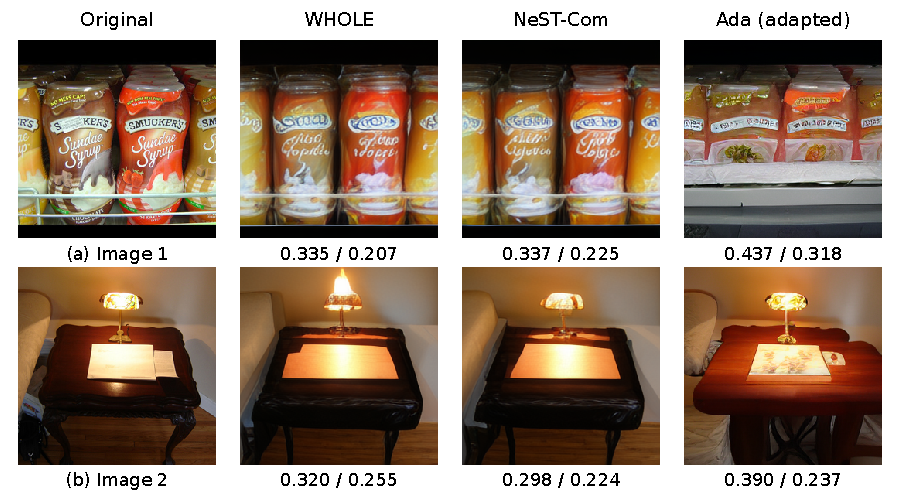
\includegraphics[width=6.0in]{supplemental/N512_previous_figure3.pdf}\end{center}
The earlier N1024 figure remains in the supplemental asset directory. The native-array identifiers, source pixel hashes, wire inputs, display-image hashes, and full-precision metrics are retained in the source map and prior selection record. No image content was enhanced or repaired.
\subsection*{Machine-readable evidence}

\href{https://github.com/daiqizai/var-comm/blob/2c303b615f73edd0a7a971308c0df8bd5bb885d0/results/nestcom_evidence_20261029_v1/e1/REPORT_zh.md}{E1 report and complete frame/source/paired data}\par
\href{https://github.com/daiqizai/var-comm/blob/2c303b615f73edd0a7a971308c0df8bd5bb885d0/results/nestcom_evidence_20261029_v1/e2/REPORT_zh.md}{E2 report and complete frame/source/paired data}\par
\href{https://github.com/daiqizai/var-comm/blob/2c303b615f73edd0a7a971308c0df8bd5bb885d0/results/nestcom_evidence_20261029_v1/statistics_identity.json}{100-source statistics identity}\par
\href{https://github.com/daiqizai/var-comm/blob/2c303b615f73edd0a7a971308c0df8bd5bb885d0/results/nestcom_n512_20261028_v1/delivery/REPORT.md}{N512 formal results and policies}\par
\href{https://github.com/daiqizai/var-comm/blob/2c303b615f73edd0a7a971308c0df8bd5bb885d0/results/wcl_revision_20261027_v1/p1_bootstrap_clarification_v1.md}{Historical mismatch: index-only bootstrap reuse clarification}\par
\href{https://github.com/daiqizai/var-comm/blob/2c303b615f73edd0a7a971308c0df8bd5bb885d0/results/five_method_timing_20261020_v1/delivery/summary_ms_per_image.csv}{Timing data}\par
\end{document}